\documentclass[a4paper,11pt]{article}
\usepackage[margin=2.4cm]{geometry}
\usepackage{ctex}
\usepackage{amsmath,amssymb}
\usepackage{booktabs}
\usepackage{multirow}
\usepackage{array}
\usepackage{makecell}
\usepackage{siunitx}
\usepackage{xcolor}
\usepackage{hyperref}
\usepackage{enumitem}
\usepackage{float}
\usepackage{graphicx}

\hypersetup{colorlinks=true, linkcolor=blue!60!black, citecolor=blue!60!black, urlcolor=blue!60!black}

\title{\textbf{YPOL Elastic Pilot:\\
全模拟全重建后物理观测量验证}}
\author{Baiting Tian \\ RIKEN 仁科中心 / DPOL 实验}
\date{2026 年 4 月 28 日}

\begin{document}
\maketitle

\section*{摘要}

本 pilot 在 ypol elastic Geant4 输出 (\texttt{ypol\_new\_20260413\_elastic\_allair}) 上跑全重建：
proton via RK 拟合 + neutron via NEBULA（位置加权重心 + ToF/$\beta$ → $|\vec p|$）。
\textbf{两端 reco 都旋转到靶系} —— rotation fix (2026-04-28) 在
\texttt{libs/analysis/include/NEBULAFrameRotation.hh} 把 NEBULA 的 lab 系 direction 旋到靶系，与 \texttt{truth\_neutron\_p4} 同坐标系。

样本：2 targets (Sn112, Sn124) × 4 gammas (g050, g060, g070, g080) × 2 helicities = 16 cells × 1000 events = 16k events。
工具：\texttt{bin/reconstruct\_target\_momentum} 重编 (commit pending) + 新增 \texttt{NEBULAFrameRotation::RotateRecoNeutronsToTargetFrame}。

\section{覆盖率与样本统计}

\begin{table}[H]
\centering\footnotesize
\caption{Per-cell 样本与基础统计 (16 cells, N=1000/cell, post-rotation-fix)}
\begin{tabular}{lllrrrrrrr}
\toprule
target & gamma & hel & N & N\_pair &
truth $\langle\Delta p_x\rangle$ & reco $\langle\Delta p_x\rangle$ &
truth $R_x$ & reco $R_x$ & reco\_full $R_x$ \\
\midrule
Sn112E190 & g050 & ynp & 1000 & 302 & +4.042 & +2.288 & +1.092 & +1.083 & +0.830 \\
Sn112E190 & g050 & ypn & 1000 & 305 & +2.562 & +1.229 & +1.088 & +1.028 & +0.955 \\
Sn112E190 & g060 & ynp & 1000 & 299 & -1.318 & -1.411 & +0.923 & +0.946 & +0.834 \\
Sn112E190 & g060 & ypn & 1000 & 350 & +3.115 & +2.519 & +1.160 & +1.132 & +1.000 \\
Sn112E190 & g070 & ynp & 1000 & 385 & -0.802 & -0.300 & +0.961 & +0.980 & +0.887 \\
Sn112E190 & g070 & ypn & 1000 & 313 & +0.171 & -0.472 & +1.016 & +0.980 & +1.087 \\
Sn112E190 & g080 & ynp & 1000 & 379 & -0.755 & -1.680 & +0.972 & +0.919 & +0.876 \\
Sn112E190 & g080 & ypn & 1000 & 386 & +0.756 & +0.673 & +1.062 & +1.033 & +0.949 \\
Sn124E190 & g050 & ynp & 1000 & 294 & +1.661 & +1.208 & +1.041 & +1.024 & +1.028 \\
Sn124E190 & g050 & ypn & 1000 & 316 & +0.917 & -0.046 & +1.041 & +1.000 & +0.915 \\
Sn124E190 & g060 & ynp & 1000 & 329 & +0.204 & +0.714 & +1.004 & +1.033 & +0.913 \\
Sn124E190 & g060 & ypn & 1000 & 363 & +2.135 & +0.905 & +1.146 & +1.070 & +0.901 \\
Sn124E190 & g070 & ynp & 1000 & 365 & +0.565 & +0.270 & +1.016 & +1.012 & +0.807 \\
Sn124E190 & g070 & ypn & 1000 & 382 & +0.896 & +0.465 & +1.070 & +1.045 & +0.810 \\
Sn124E190 & g080 & ynp & 1000 & 353 & +0.207 & -0.906 & +1.012 & +0.942 & +0.783 \\
Sn124E190 & g080 & ypn & 1000 & 409 & +1.012 & -1.207 & +1.058 & +0.931 & +0.810 \\
\bottomrule
\end{tabular}
\end{table}

\textbf{读法}：$\langle\Delta p_x\rangle$ = $(p_{x,p} - p_{x,n})$ 的事件中位 (MeV/$c$)，
对 reco 列采用 reco\_proton + (reco\_neutron 若有, 否则 truth\_neutron 代理)。
$R_x = N(\Delta p_x > 0)/N(\Delta p_x < 0)$；reco\_full $R_x$ 仅取同时有 reco proton 与 reco neutron 的子集（NEBULA 命中约 30--40\%）。
\textbf{rotation fix 后} reco neutron 的 $\Delta p_x$ 系统偏置从 $-31.6$ MeV/$c$ 降到 $+0.71$ MeV/$c$（library 修复 2026-04-28，库代码 \texttt{libs/analysis/include/NEBULAFrameRotation.hh}）。

\begin{figure}[H]
\centering
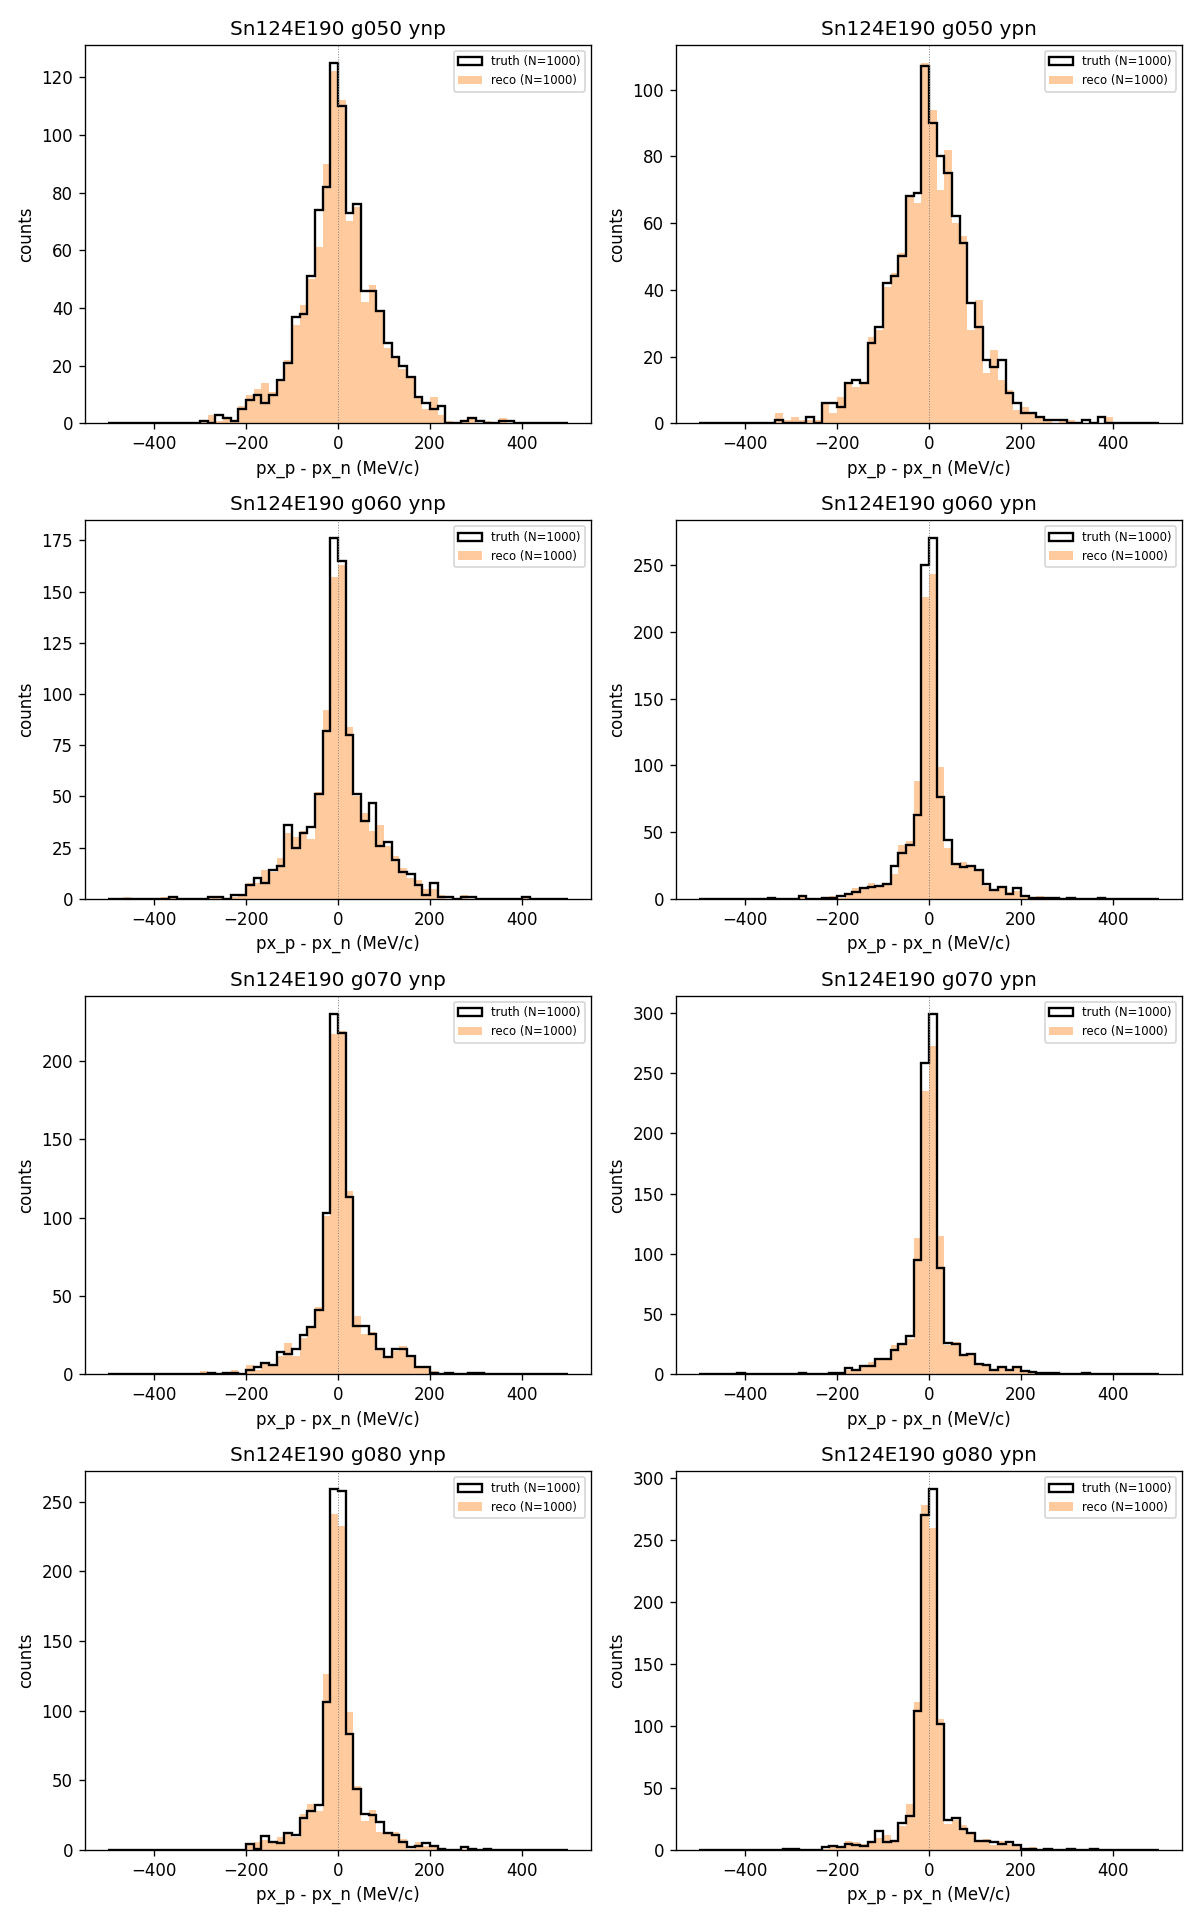
\includegraphics[width=0.95\textwidth]{figures/ypol_phys/px_diff_hist_Sn124E190.png}
\caption{$\Delta p_x = p_{x,p} - p_{x,n}$ 分布 (Sn124E190, 4 cell)。黑线 = truth, 填色 = reco。reco 应跟随 truth 形状但带 reco 端 smearing。}
\end{figure}
\begin{figure}[H]
\centering
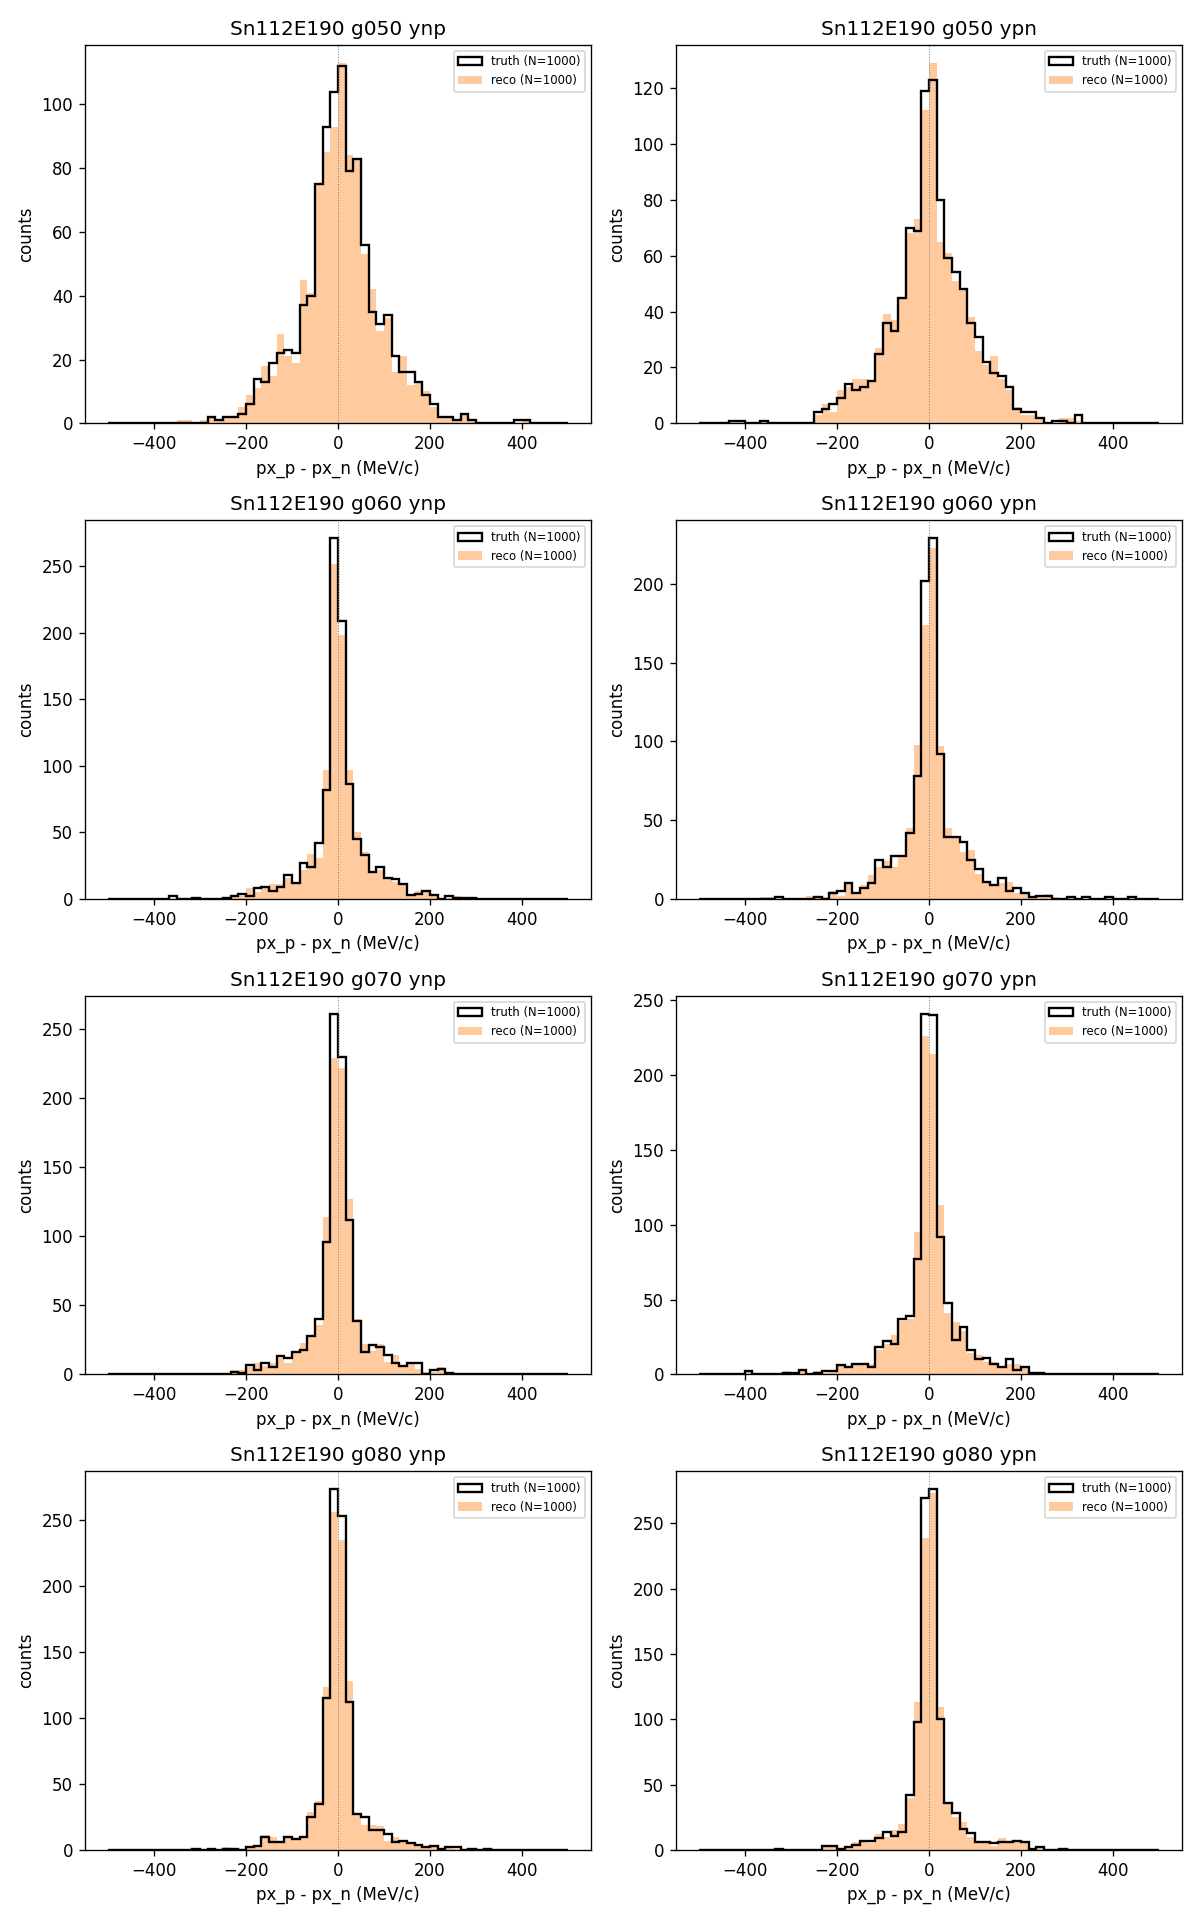
\includegraphics[width=0.95\textwidth]{figures/ypol_phys/px_diff_hist_Sn112E190.png}
\caption{同图但 Sn112E190 target。}
\end{figure}
\begin{figure}[H]
\centering
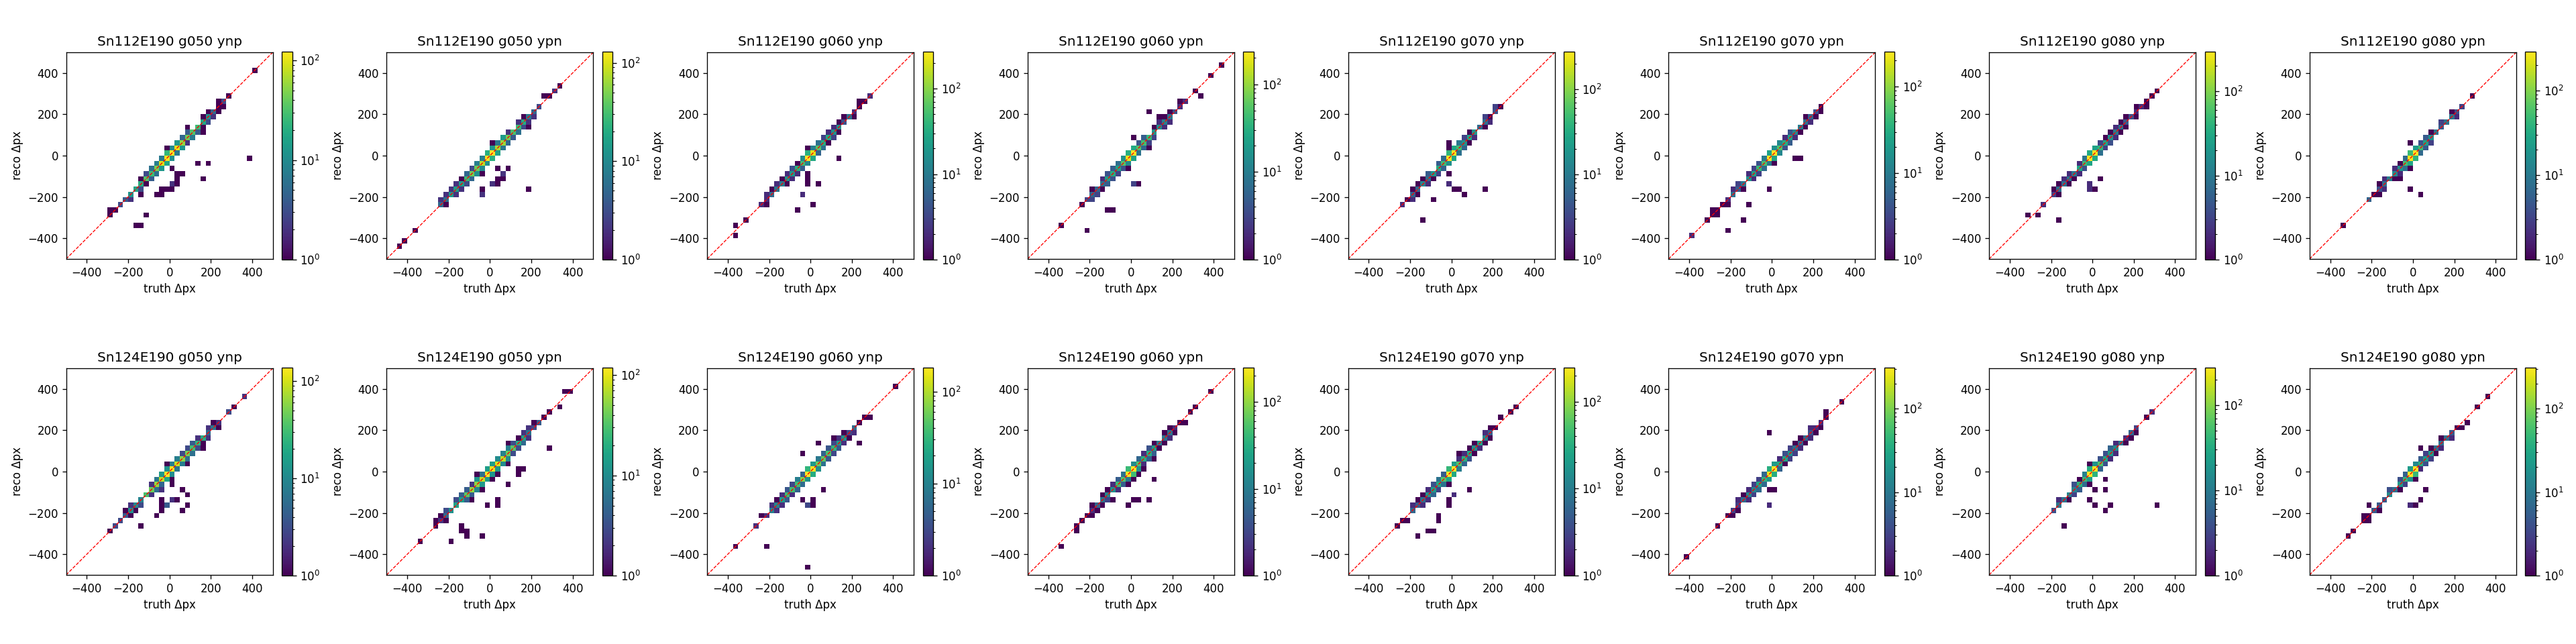
\includegraphics[width=0.95\textwidth]{figures/ypol_phys/px_diff_truth_vs_reco_hist2d.png}
\caption{$\Delta p_x$ 的 truth (横) vs reco (纵) 二维直方图，每 cell 一格。对角线 = 完美重建。}
\end{figure}
\begin{figure}[H]
\centering
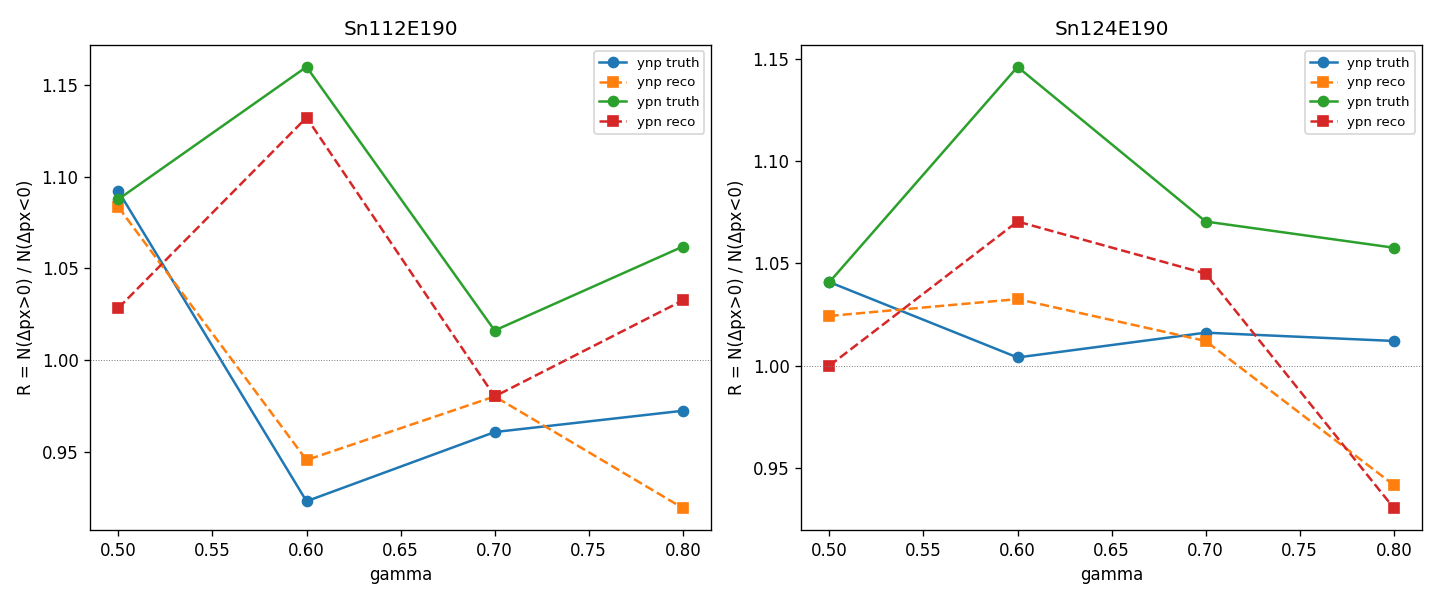
\includegraphics[width=0.95\textwidth]{figures/ypol_phys/r_vs_gamma.png}
\caption{$R_x = N_+/N_-$ 随 gamma 的趋势。两 panel = 两 target；线/标 = helicity；实线 = truth, 虚线 = reco。reco 对 truth 趋势的保留程度即全重建对极化分析的 fidelity。}
\end{figure}
\section{结论}

\begin{enumerate}[nosep]
\item \textbf{(px\_p − px\_n) 不对称信号}：见上表 $\langle\Delta p_x\rangle$ 列对比 truth vs reco。
\item \textbf{R/gamma 趋势}：见 \texttt{r\_vs\_gamma.png}。reco 与 truth 同方向变化即"reco 没毁掉信号"。
\item \textbf{下一步}：若趋势可见，扩大到 8 gamma + 全 190k events / cell。若不可见，说明 reco fidelity 不够，需要回到详细版报告 §10 的 P0 修复（Bethe-Bloch + Kalman MS）。
\end{enumerate}
\end{document}
